\documentclass{standalone}
\usepackage{tikzducks}
\usepackage[osf]{AlegreyaSans}
\begin{document}
%\tikz\duck[davidlikespineapplepizza];

\makeatletter \def\niafactor{0.3} \def\yshiftfactor{-1.4cm}
\begin{tikzpicture}
\node at (2,0) {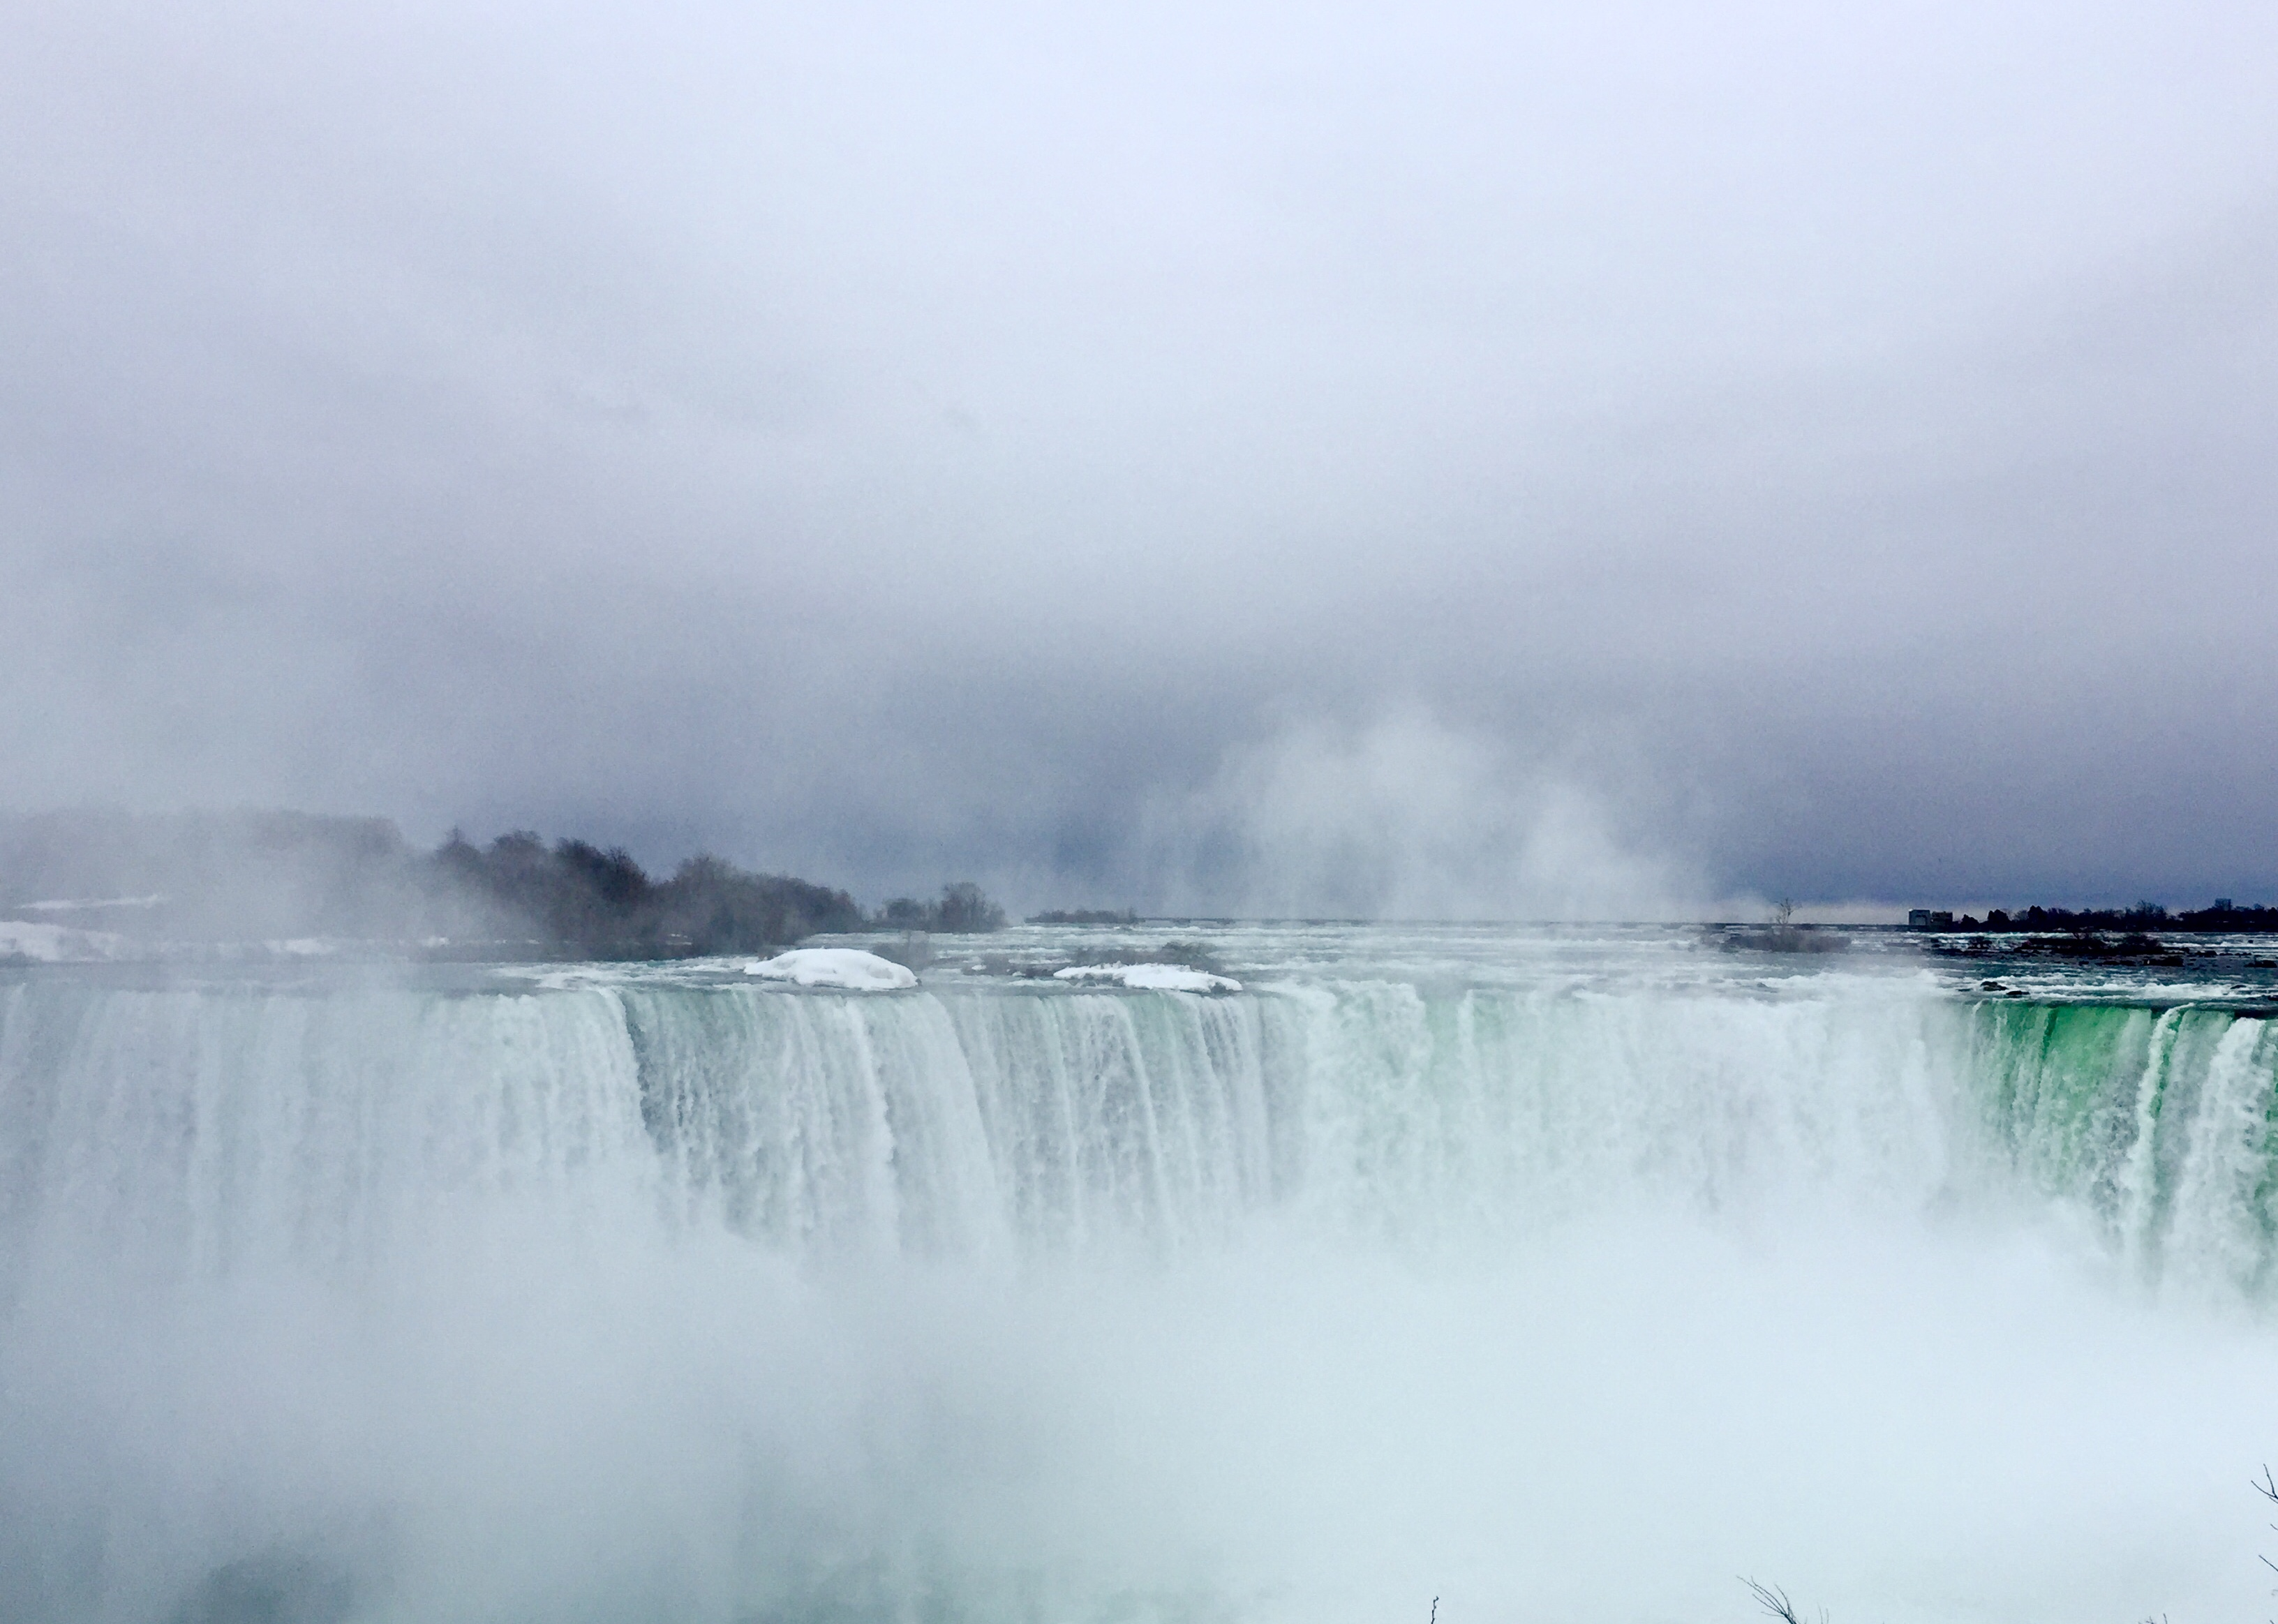
\includegraphics[width=20cm]{niagara}};
\node[font=\sffamily\bfseries\huge\color{white}] at (2,-4) {More exciting than a bathtub!};
\begin{scope}[yshift=\yshiftfactor,xshift=-1.9cm,xscale=-1]
\begin{scope}[scale=\niafactor]
\duck[mullet=red,sunglasses];
\begin{pgfinterruptboundingbox}
    \fill[red] \duckpathmullet;
  \end{pgfinterruptboundingbox}
\end{scope}
\end{scope}
\begin{scope}[yshift=\yshiftfactor,xshift=0.5cm]
\begin{scope}[scale=\niafactor]
\duck[mullet=red,sunglasses];
\begin{pgfinterruptboundingbox}
    \fill[red] \duckpathmullet;
  \end{pgfinterruptboundingbox}
\end{scope}
\end{scope}
\begin{scope}[yshift=\yshiftfactor,xshift=3cm]
\begin{scope}[scale=\niafactor]
\duck[mullet=red,sunglasses];
\begin{pgfinterruptboundingbox}
    \fill[red] \duckpathmullet;
  \end{pgfinterruptboundingbox}
\end{scope}
\end{scope}
\begin{scope}[yshift=\yshiftfactor,xshift=6cm]
\begin{scope}[scale=\niafactor]
\duck[mullet=red,sunglasses];
\begin{pgfinterruptboundingbox}
    \fill[red] \duckpathmullet;
  \end{pgfinterruptboundingbox}
\end{scope}
\end{scope}
\begin{scope}[yshift=\yshiftfactor,xshift=8.5cm]
\begin{scope}[scale=\niafactor]
\duck[mullet=red,sunglasses];
\begin{pgfinterruptboundingbox}
    \fill[red] \duckpathmullet;
  \end{pgfinterruptboundingbox}
\end{scope}
\end{scope}


\end{tikzpicture}

%\quad
%\begin{tikzpicture}
%\duck[darthvader=blue,squareglasses];\def\yscalefactor{1}
%  \fill[brown!50!black,rotate=-17] (0.43,1.8) rectangle (0.8,1.84);
%  \fill[brown!50!black,rotate=-17] (0.12,1.8) rectangle (0.22,1.84);
%  \fill[brown!50!black,rotate=-20,rounded corners=\yscalefactor*2] (-0.16,1.62) -- (-0.18,1.85) -- (0.05,1.87) -- (0.04,1.62) -- cycle
%   %[rounded corners=\yscalefactor*1.5] (-0.14,1.64) -- (-0.16,1.83) -- (0.03,1.85) -- (0.02,1.64) -- cycle
%   ;
%  \fill[brown!50!black,rotate=-20,rounded corners=\yscalefactor*2,even odd rule] (0.12,1.63) -- (0.10,1.88) -- (0.36,1.90) -- (0.35,1.65) -- cycle
%   %[rounded corners=\yscalefactor*1.5] (0.14,1.65) -- (0.12,1.86) -- (0.34,1.88) -- (0.33,1.67) -- cycle
%   ;
%  \path (0.1,0.1) rectangle (2.1,2.22);
%  \begin{pgfinterruptboundingbox}
%    \fill[\duck@darthvader] \duckpathdarthvader;
%  \end{pgfinterruptboundingbox}
%\end{tikzpicture}

\end{document} 